\documentclass{beamer}
\usepackage[utf8]{inputenc}
\usepackage[english]{babel}
\usepackage{helvet}
\usepackage[T1]{fontenc}
\usepackage{textcomp}
\usepackage[inline]{asymptote}
\usepackage{slide_helper}
\usepackage{multirow}
\usepackage{cellspace}
\usepackage{tikz}
\usepackage{fp}
\usepackage{cancel}
\usepackage{subfigure}
\usetikzlibrary{shapes.geometric, arrows}
\usepackage{pgfplots}
\pgfplotsset{compat=1.5} 
\usepgfplotslibrary{statistics}
\usetikzlibrary{external}
\tikzexternalize%

\title[MA205 - Section 3.2]{Conditional Probability}

\DeclareSymbolFont{extraup}{U}{zavm}{m}{n}
\DeclareMathSymbol{\varheart}{\mathalpha}{extraup}{86}
\DeclareMathSymbol{\vardiamond}{\mathalpha}{extraup}{87}
\DeclareMathSymbol{\varclub}{\mathalpha}{extraup}{84} 
\DeclareMathSymbol{\varspade}{\mathalpha}{extraup}{85}

\newcommand{\suitheart}[1][]{{\color{red}\text{#1}\varheart}}
\newcommand{\suitspade}[1][]{{\color{black}\text{#1}\spadesuit}}
\newcommand{\suitdiamond}[1][]{{\color{red}\text{#1}\vardiamond}}
\newcommand{\suitclub}[1][]{{\color{black}\text{#1}\varclub}}
\newcommand{\card}[2]{{#1{\color{black}\text{#2}}}}

\newcommand{\prob}[1]{P\left({#1}\right)}
\newcommand{\jointprob}[3]{\prob{{#1}~\text{#2}~{#3}}}
\newcommand{\condprob}[2]{\prob{{#1}~|~{#2}}}
\newcommand{\comb}[2]{_{#1}C_{#2}}

\newcommand\encircle[1]{%
  \tikz[baseline=(X.base)]  % chktex 36 chktex 1
    \node (X) [draw, shape=circle, inner sep=0, fill=yellow!10] {\strut #1};} % chktex 36 chktex 1

\begin{document}
\begin{frame}
\titlepage
\end{frame}

\begin{frame}
\begin{example}\label{ML classifier}
\vspace{-2mm}%beamer bug: extra space is added when a label is used, so this is to make this slide and the next look the same
The \dataset{photo\_classify} data set represents a machine learning algorithm classifying a sample of 1822 photos as either about fashion or not.\pause

\vspace{-1mm}
\begin{center}
\begin{tabular}{llccc}
&&\multicolumn{2}{c}{\variable{truth}} & \\\cline{3-4}
&&\outcome{fashion} & \outcome{not} & Total \\\cline{2-5}
\multirow{2}{*}{\variable{mach\_learn}} & \outcome{pred\_fashion} & 197 & 22 & 219 \\
&\outcome{pred\_not}& 112 & 1491 & 1603 \\\cline{2-5}
&Total & 309 & 1513 & 1822
\end{tabular}
\end{center}\pause

\question{If a photo is actually about fashion, what is the chance the algorithm will correctly identify the photo as being about fashion?}\pause
\answer{Of the 309 fashion photos, the algorithm correctly classifies 197 of them.

\vspace{-7mm}
\begin{equation*}
\jointprob{\text{\small\variable{mach\_learn} is \outcome{pred\_fashion}}}{given}{\text{\small\variable{truth} is \outcome{fashion}}}=\dfrac{197}{309} = 0.638
\end{equation*}}
\vspace{-5mm}
\end{example}
\end{frame}

\begin{frame}
\begin{example}
Using the same data set as in Example~\ref{ML classifier}.
\vspace{-2mm}
\begin{center}
\begin{tabular}{llccc}
&&\multicolumn{2}{c}{\variable{truth}} & \\\cline{3-4}
&&\outcome{fashion} & \outcome{not} & Total \\\cline{2-5}
\multirow{2}{*}{\variable{mach\_learn}} & \outcome{pred\_fashion} & 197 & 22 & 219 \\
&\outcome{pred\_not}& 112 & 1491 & 1603 \\\cline{2-5}
&Total & 309 & 1513 & 1822
\end{tabular}
\end{center}

\question{If the algorithm predicts the photo as being about fashion, what is the probability is actually is?}\pause
\answer{Of the 1603 photos predicted to be about fashion, 112 we actually about fashion.

\vspace{-7mm}
\begin{equation*}
\jointprob{\text{\small\variable{truth} is \outcome{fashion}}}{given}{\text{\small\variable{mach\_learn} is \outcome{pred\_fashion}}}=\dfrac{197}{219} = 0.900
\end{equation*}}
\vspace{-5mm}
\end{example}
\end{frame}

\begin{frame}
\begin{note}
It can be helpful to draw Venn Diagrams of these contingency tables using rectangles.
\end{note}\pause

\begin{example}
The Venn Diagram for Example~\ref{ML classifier} is:
\begin{center}
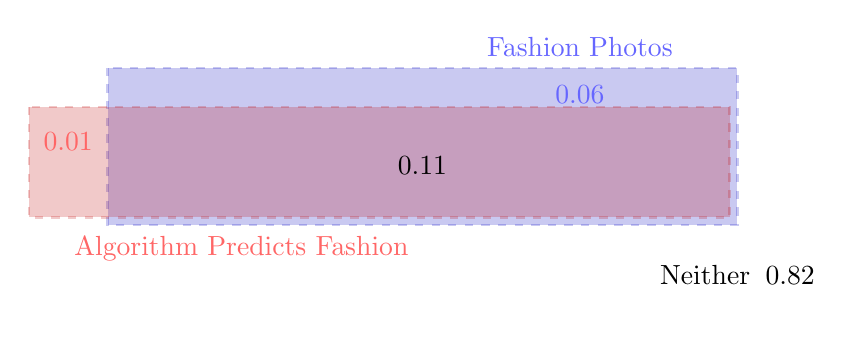
\begin{tikzpicture}
\draw[draw, dashed, fill=blue!40, blue!75!black, opacity=0.21, thick] (0,0) rectangle (8,-2);
\draw[draw, dashed, fill=red!40, red!75!black, opacity=0.21, thick] (-1,-0.5) rectangle (7.9,-1.9);
\node [label={[blue!60] Fashion Photos}] at (6,-0.1) {};
\node [label={[red!60] Algorithm Predicts Fashion}] at (1.7,-2.7) {};
\node [label={[red!60] 0.01}] at (-0.5,-1.3) {};
\node [label={[blue!60] 0.06}] at (6,-.7) {};
\node [label={[black] 0.11}] at (4,-1.6) {};
\node [label={[black] Neither\: 0.82}] at (8,-3) {};
\end{tikzpicture}
\end{center}
\end{example}
\end{frame}

\begin{frame}
\begin{definition}
A \textbf{marginal probability} is a probability based on a single variable without regard to other variables.
\end{definition}\pause

\begin{example}
\begin{equation*}
\prob{\text{\variable{mach\_learn} is \outcome{pred\_fashion}}} = \dfrac{219}{1822} = 0.12
\end{equation*}\pause
\vspace{-3.5mm}
\end{example}

\begin{definition}
A probability of outcomes for two or more variables is called a\\ \textbf{joint probability}.
\end{definition}\pause

\begin{example}
\vspace{-4mm}
\begin{equation*}
\jointprob{\text{\variable{mach\_learn} is \outcome{pred\_fashion}}}{and}{\text{\variable{truth} is \outcome{fashion}}} = \dfrac{197}{1822} = 0.11
\end{equation*}
\vspace{-4.5mm}
\end{example}
\end{frame}

\begin{frame}
\begin{note}
Sometimes a comma is substituted for \textquote{and} in a joint probability.

\vspace{-1mm}
\begin{center}
\begin{tabular}{c}
$\prob{\small\text{\variable{mach\_learn} is \outcome{pred\_fashion}, \variable{truth} is \outcome{fashion}}}$ \\
means the same thing as \\
$\jointprob{\small\text{\variable{mach\_learn} is \outcome{pred\_fashion}}}{and}{\text{\variable{truth} is \outcome{fashion}}}$
\end{tabular}
\end{center}
\end{note}
\end{frame}

\begin{frame}
\begin{definition}
A \textbf{table proportions} is a table that summarizes joint probabilities. The proportions are computed by dividing each count by table's total.
\end{definition}\pause

\begin{example}\label{table props}
\vspace{-2mm}%beamer bug: extra space is added when a label is used, so this is to make this slide and the next look the same
The table proportions for \dataset{photo\_classify} are:

\vspace{-5mm}
\begin{center}
%\addtolength{\cellspacetoplimit}{1.5pt}
%\addtolength{\cellspacebottomlimit}{1.5pt}
\begin{tabular}{Sl Sr Sr Sr}\hline
& \variable{truth}: \outcome{fashion} & \variable{truth}: \outcome{not} & Total \\\hline
\variable{mach\_learn}: \outcome{pred\_fashion} & $\tfrac{197}{1822}$  & \visible<3->{$\tfrac{22}{1822}$} & \visible<4->{$\tfrac{219}{1822}$} \\[1mm]
\variable{mach\_learn}: \outcome{pred\_not} & \visible<5->{$\tfrac{112}{1822}$} & \visible<6->{$\tfrac{1491}{1822}$} & \visible<7->{$\tfrac{1603}{1822}$} \\\hline
Total & \visible<8->{$\tfrac{309}{1822}$} & \visible<9->{$\tfrac{1513}{1822}$} & \visible<10->{$\tfrac{1822}{1822}$} \\\hline
\multicolumn{4}{c}{$\downarrow~\downarrow~\downarrow$}\\\hline
& \variable{truth}: \outcome{fashion} & \variable{truth}: \outcome{not} & Total \\\hline
\variable{mach\_learn}: \outcome{pred\_fashion} & 0.1081  & \visible<3->{0.0121} & \visible<4->{0.1202} \\
\variable{mach\_learn}: \outcome{pred\_not} & \visible<5->{0.0615} & \visible<6->{0.8183} & \visible<7->{0.8798} \\\hline
Total & \visible<8->{0.1696} & \visible<9->{0.8304} & \visible<10->{1.0} \\\hline
\end{tabular}
\end{center}
\end{example}
\end{frame}

\begin{frame}
\begin{example}
The table proportions from Example~\ref{table props} make a probability distribution.
\begin{center}
\begin{tabular}{lc}\hline
Joint Outcome & Probability \\\hline
\variable{mach\_learn} is \outcome{pred\_fashion} and  \variable{truth} is \outcome{fashion} & 0.1081 \\
\variable{mach\_learn} is \outcome{pred\_fashion} and  \variable{truth} is \outcome{not} & 0.0121\\
\variable{mach\_learn} is \outcome{pred\_not} and  \variable{truth} is \outcome{fashion} & 0.0615\\
\variable{mach\_learn} is \outcome{pred\_not} and  \variable{truth} is \outcome{not} & 0.8182\\\hline
\end{tabular}
\end{center}
\end{example}\pause

\begin{note}
Joint probabilities can be used to calculate marginal probabilities in simple cases.
\end{note}\pause

\begin{example}\small
\vspace{-4mm}
\begin{equation*}
\begin{aligned}
\prob{\small\text{\variable{truth} is \outcome{fashion}}}
&= \jointprob{\text{\small\variable{mac\_learn} is \outcome{pred\_fashion}}}{and}{\text{\small\variable{truth} is \outcome{fashion}}} \\
&\qquad +\jointprob{\text{\small\variable{mac\_learn} is \outcome{pred\_not}}}{and}{\text{\small\variable{truth} is \outcome{fashion}}} \\\pause
&=0.1081 + 0.0615 \pause
= 0.1696
\end{aligned}
\end{equation*}
\end{example}
\end{frame}

\begin{frame}
\begin{definition}
A \textbf{conditional probability} is a probability computed under a condition.
\end{definition}\pause

\begin{example}
\vspace{-4mm}
\begin{equation*}
\prob{\text{\small\variable{truth} is \outcome{fashion} given \variable{mach\_learn} is \outcome{pred\_fashion}}}=\dfrac{197}{219} = 0.900
\end{equation*}
\end{example}\pause

\begin{definition}
There are two parts to a conditional probability, the \textbf{outcome of interest} and the \textbf{condition}.
\vspace{-3mm}
\begin{equation*}
\begin{array}{c}
\prob{\text{outcome of interest given condition}}\\
\text{is the same as}\\
\condprob{\text{outcome of interest}}{\text{condition}}
\end{array}
\end{equation*}
\end{definition}\pause

\begin{example}
\vspace{-4mm}
\begin{equation*}
\condprob{\text{\small\variable{truth} is \outcome{fashion}}}{\text{\small\variable{mach\_learn} is \outcome{pred\_fashion}}}=\dfrac{197}{219} = 0.900
\end{equation*}
\end{example}
\end{frame}

\begin{frame}
\begin{note}
Conditional probabilities are computed as:
\begin{equation*}
\condprob{A}{B} = \dfrac{\jointprob{A}{and}{B}}{\prob{B}}
\end{equation*}
\end{note}\pause

\begin{example}
\begin{equation*}
\begin{array}{l}
\condprob{\text{\small\variable{truth} is \outcome{fashion}}}{\text{\small\variable{mach\_learn} is \outcome{pred\_fashion}}}\\[2mm]
\qquad= \dfrac{\jointprob{\text{\small\variable{truth} is \outcome{fashion}}}{and}{\text{\small\variable{mach\_learn} is \outcome{pred\_fashion}}}}{\prob{\text{\small\variable{mach\_learn} is \outcome{pred\_fashion}}}}\\[2mm]
\qquad=\dfrac{0.0615}{0.1696} \\[3mm]
\qquad= 0.3626
\end{array}
\end{equation*}
\end{example}
\end{frame}

\begin{frame}
\begin{example}
The \dataset{smallpox} data set provides a sample of 6,224 individuals from the year 1721 who were exposed to smallpox in Boston.
\begin{center}\small
\begin{tabular}{llrrrcrrr}
&&\multicolumn{2}{c}{\variable{inoculated}} & & &\multicolumn{2}{c}{\variable{inoculated}} & \\\cline{3-4}\cline{7-8}
&&\outcome{yes}&\outcome{no}&Total &&\outcome{yes}&\outcome{no}&Total  \\\cline{2-5}\cline{7-9}
\multirow{2}{*}{\variable{result}} & \outcome{lived} & 238 & 5136 & 5374 && 0.0382 & 0.8252 & 0.8634  \\
&\outcome{died} & 6 & 844 & 850 && 0.0010 & \color<5>{red!75}{0.1356} & 0.1366 \\\cline{2-5}\cline{7-9}
&Total & 244 & 5980 & 6224 && 0.0392 & \color<5>{blue!75}{0.9608} & 1.0000
\end{tabular}
\end{center}\pause
\question{What is the probability that a randomly selected person who was not inoculated died from smallpox?}\pause
\answer{%
\vspace{-2mm}
\begin{equation*}
\begin{array}{l}
\condprob{\text{\small\variable{result} is \outcome{died}}}{\text{\variable{inoculated} is \outcome{no}}} \\[2mm]\pause\qquad=\dfrac{\jointprob{\text{\small\variable{result} is \outcome{died}}}{and}{\text{\small\variable{inoculated} is \outcome{no}}}}{\prob{\text{\small\variable{inoculated} is \outcome{no}}}} \\\pause
\qquad=\dfrac{\color<5>{red!65}{0.1356}}{\color<5>{blue!65}{0.9608}} \\[4mm]\pause
\qquad=0.1411\approx 14.11\%
\end{array}
\end{equation*}}
\vspace{-3mm}
\end{example}
\end{frame}

\begin{frame}
\begin{example}
The \dataset{smallpox} data set provides a sample of 6,224 individuals from the year 1721 who were exposed to smallpox in Boston.
\begin{center}\small
\begin{tabular}{llrrrcrrr}
&&\multicolumn{2}{c}{\variable{inoculated}} & & &\multicolumn{2}{c}{\variable{inoculated}} & \\\cline{3-4}\cline{7-8}
&&\outcome{yes}&\outcome{no}&Total &&\outcome{yes}&\outcome{no}&Total  \\\cline{2-5}\cline{7-9}
\multirow{2}{*}{\variable{result}} & \outcome{lived} & 238 & 5136 & 5374 && 0.0382 & 0.8252 & 0.8634  \\
&\outcome{died} & 6 & 844 & 850 && \color<5>{red!75}{0.0010} & 0.1356 & 0.1366 \\\cline{2-5}\cline{7-9}
&Total & 244 & 5980 & 6224 && \color<5>{blue!75}{0.0392} & 0.9608 & 1.0000
\end{tabular}
\end{center}\pause
\question{What is the probability that a randomly selected inoculated person died from smallpox?}\pause
\answer{%
\vspace{-2mm}
\begin{equation*}
\begin{array}{l}
\condprob{\text{\small\variable{result} is \outcome{died}}}{\text{\variable{inoculated} is \outcome{yes}}} \\[2mm]\pause\qquad=\dfrac{\jointprob{\text{\small\variable{result} is \outcome{died}}}{and}{\text{\small\variable{inoculated} is \outcome{yes}}}}{\prob{\text{\small\variable{inoculated} is \outcome{yes}}}} \\\pause
\qquad=\dfrac{\color<5>{red!65}{0.0010}}{\color<5>{blue!65}{0.0392}} \\[4mm]\pause
\qquad=0.0255\approx 2.55\%
\end{array}
\end{equation*}}
\vspace{-3mm}
\end{example}
\end{frame}

\begin{frame}
\begin{example}
The \dataset{smallpox} data set provides a sample of 6,224 individuals from the year 1721 who were exposed to smallpox in Boston.

\vspace{2mm}
The residents of Boston self-selected whether or not to be inoculated.

\vspace{2mm}
\question{Is this study observational or experimental?}\pause\answersingleline{Observational}\pause

\vspace{2mm}
\question{Can we infer any causal connection using this data?}\pause
\answer{No, the fact this is an observational study combined with the self-selecting bias means we cannot.}\pause

\vspace{2mm}
\question{What are some potential confounding variables that might influence whether someone \outcome{lived} or \outcome{died}?}\pause
\answer{People die for many reasons, wealth determines level of medical care available, etc\ldots}
\end{example}
\end{frame}

\begin{frame}
\begin{block}{General Multiplication Rule}
If $A$ and $B$ represent two outcomes or events, then
\begin{equation*}
\jointprob{A}{and}{B} = \condprob{A}{B}\cdot\prob{B}
\end{equation*}
\end{block}\pause

\begin{example}
Suppose we are only given two pieces of information: 
\begin{itemize}
\item 96.08\% of Boston residents were not inoculated.
\item 85.88\% of Boston residents who were not inoculated ended up surviving.
\end{itemize}
Let us find the probability that a resident who was no inoculated  and lived.\pause

\vspace{-5mm}
\begin{equation*}
\begin{array}{l}
\jointprob{\text{\small\variable{result} is \outcome{lived}}}{and}{\text{\small\variable{inoculated} is \outcome{no}}} \\\pause
\qquad= \condprob{\text{\small\variable{result} is \outcome{lived}}}{\text{\small\variable{inoculated} is \outcome{no}}} \cdot \prob{\text{\small\variable{inoculated} is \outcome{no}}}\\\pause
\qquad= 0.8588 \cdot 0.9698\\\pause
\qquad= 0.8251 \approx 82.51\%
\end{array}
\end{equation*}
\end{example}
\end{frame}

\begin{frame}
\begin{example}
Let's use
\begin{itemize}
\item $\prob{\text{\small\variable{inoculated} is \outcome{yes}}}=0.0392$
\item $\condprob{\text{\small\variable{result} is \outcome{lived}}}{\text{\small\variable{inoculated} is \outcome{yes}}}=0.9754$
\end{itemize}
to find the probability that a person was both inoculated and lived.\pause

\vspace{-5mm}
\begin{equation*}
\begin{array}{l}
\jointprob{\text{\small\variable{result} is \outcome{lived}}}{and}{\text{\small\variable{inoculated} is \outcome{yes}}} \\\pause
\qquad= \condprob{\text{\small\variable{result} is \outcome{lived}}}{\text{\small\variable{inoculated} is \outcome{yes}}} \cdot \prob{\text{\small\variable{inoculated} is \outcome{yes}}}\\\pause
\qquad= 0.0382 \cdot 0.9754\\\pause
\qquad= 0.0382 \approx 3.82\%
\end{array}
\end{equation*}
\end{example}
\end{frame}

\begin{frame}
\begin{block}{Sum of Conditional Probabilities}
Let $A_1$, $A_2$, \ldots, $A_k$ represent all the disjoint outcomes for a variable. Then if $B$ is an event, possibly for another variable, we have:
\begin{equation*}
\condprob{A_1}{B} + \condprob{A_2}{B} + \cdots + \condprob{A_k}{B}  = 1
\end{equation*}
\end{block}\pause

\begin{note}
If an event and it's complement are conditioned on the same information, then:
\begin{equation*}
\condprob{A}{B} = 1 - \condprob{A^C}{B}
\end{equation*}
\end{note}\pause

\begin{example}
\question{If 97.54\% of the inoculated people lived, what is the proportion of people that must have died?}\pause
\answer{There are only two outcomes: \outcome{lived} and \outcome{died}. Which means that $100\% - 97.54\% = 2.46\%$ people who were inoculated died.}
\end{example}
\end{frame}

\begin{frame}
\begin{example}
Let $X$ and $Y$ represent the outcomes of rolling two dice.

\vspace{2mm}
Let us compute the following:
\begin{equation*}
\begin{array}{ll}
\condprob{Y=1}{X=1} \pause
&= \dfrac{\jointprob{Y=1}{and}{X=1}}{\prob{X=1}} \\\pause
&= \dfrac{\prob{Y=1}\cdot\prob{X=1}}{\prob{X=1}} \\\pause
&= \dfrac{\prob{Y=1}\cdot\cancel{\prob{X=1}}}{\cancel{\prob{X=1}}} \\\pause
&= \prob{Y=1}
\end{array}
\end{equation*}
\end{example}\pause

\begin{note}
We have shown that if two events are independent, then knowing the outcome of one should provide no information about the other.
\end{note}
\end{frame}

\begin{frame}
\begin{example}
Ron is watching a roulette table in a casino and notices that the last five outcomes were \outcome{black}. He figures that the chances of getting \outcome{black} six times in  a row is very small and puts his paycheck on red.

\vspace{2mm}
\question{Why is this a really bad idea?}\pause

\answer{Each spin of a roulette wheel is independent of any of the previous spins. The next spin has the exact same probability of getting black and any other.}
\end{example}\pause

\begin{note}
Posting the last several outcomes of a betting game is a real practice casinos use to trick people into believing the odds are in their favor. It's known as the \textbf{gambler's fallacy}.
\end{note}
\end{frame}

\begin{frame}
\begin{definition}
A \textbf{tree diagram} is a tool to organize outcomes and probabilities around the structure of the data.

\vspace{2mm}
They are most useful when two or more processes occur in a sequence and each process is conditioned on its predecessor.
\end{definition}\pause

\begin{example}
Here is the tree diagram for \dataset{smallpox} dataset.

\vspace{-2.5mm}
\begin{center}
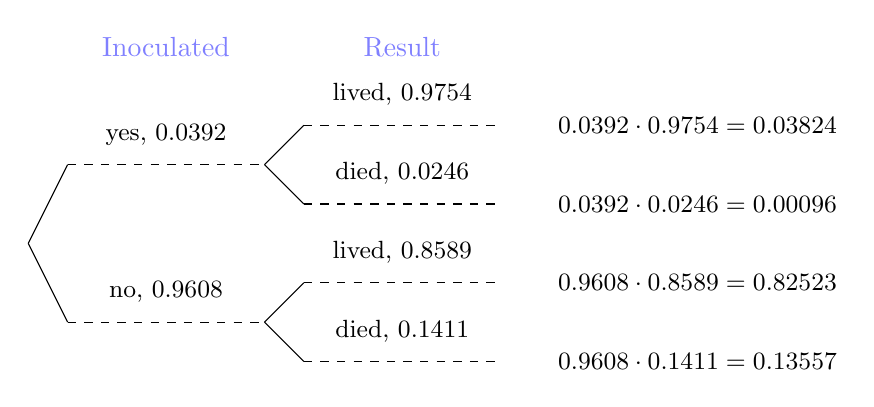
\begin{tikzpicture}
\newcommand{\varA}{\variable{Inoculated}}
\newcommand{\varB}{\variable{Result}}
\newcommand{\outAone}{\outcome{yes}}
\newcommand{\outAtwo}{\outcome{no}}
\newcommand{\outBone}{\outcome{lived}}
\newcommand{\outBtwo}{\outcome{died}}
\newcommand{\outAoneprob}{0.0392}
\newcommand{\outAtwoprob}{0.9608}
\newcommand{\outAoneBoneprob}{0.9754}
\newcommand{\outAoneBtwoprob}{0.0246}
\newcommand{\outAtwoBoneprob}{0.8589}
\newcommand{\outAtwoBtwoprob}{0.1411}

\newcommand{\rowlabel}{2.5}
\newcommand{\rowthreeup}{1.5}
\newcommand{\rowtwoup}{1.0}
\newcommand{\rowoneup}{0.5}
\newcommand{\rowonedown}{-0.5}
\newcommand{\rowtwodown}{-1.0}
\newcommand{\rowthreedown}{-1.5}

\newcommand{\colone}{0.5}
\newcommand{\coltwo}{3}
\newcommand{\colthree}{3.5}
\newcommand{\colfour}{6}
\newcommand{\colfive}{8.5}

\FPeval\midone{clip((\colone+\coltwo)/2)} % chktex 36
\FPeval\midtwo{clip((\colthree+\colfour)/2)} % chktex 36
\FPeval\ansa{clip(\outAoneprob * \outAoneBoneprob)} 
\FPeval\ansa{round(ansa:5)}
\FPeval\ansb{clip(\outAoneprob * \outAoneBtwoprob)} 
\FPeval\ansb{round(ansb:5)}
\FPeval\ansc{clip(\outAtwoprob * \outAtwoBoneprob)} 
\FPeval\ansc{round(ansc:5)}
\FPeval\ansd{clip(\outAtwoprob * \outAtwoBtwoprob)} 
\FPeval\ansd{round(ansd:5)}

\draw (0,0) -- (\colone, \rowtwoup);
\draw[dashed] (\colone, \rowtwoup) -- (\coltwo, \rowtwoup);
\draw (\coltwo, \rowtwoup) -- (\colthree, \rowthreeup);
\draw[dashed] (\colthree, \rowthreeup) -- (\colfour, \rowthreeup);
\draw (\coltwo, \rowtwoup) -- (\colthree, \rowoneup);
\draw[dashed] (\colthree, \rowoneup) -- (\colfour, \rowoneup);

\draw (0,0) -- (\colone, \rowtwodown);
\draw[dashed] (\colone, \rowtwodown) -- (\coltwo, \rowtwodown);
\draw (\coltwo, \rowtwodown) -- (\colthree, \rowthreedown);
\draw[dashed] (\colthree, \rowthreedown) -- (\colfour, \rowthreedown);
\draw (\coltwo, \rowtwodown) -- (\colthree, \rowonedown);
\draw[dashed] (\colthree, \rowonedown) -- (\colfour, \rowonedown);

\node[label={\small \outAone,~\outAoneprob}] at (\midone,\rowtwoup) {};
\node[label={\small \outAtwo,~\outAtwoprob}] at (\midone,\rowtwodown) {};
\node[label={\small \outBone,~\outAoneBoneprob}] at (\midtwo,\rowthreeup) {};
\node[label={\small \outBtwo,~\outAoneBtwoprob}] at (\midtwo,\rowoneup) {};
\node[label={\small \outBtwo,~\outAtwoBtwoprob}] at (\midtwo,\rowthreedown) {};
\node[label={\small \outBone,~\outAtwoBoneprob}] at (\midtwo,\rowonedown) {};

\node at (\colfive,\rowthreeup) {\small $\outAoneprob \cdot \outAoneBoneprob=\ansa$};
\node at (\colfive,\rowoneup) {\small $\outAoneprob \cdot \outAoneBtwoprob=\ansb$};
\node at (\colfive,\rowonedown) {\small $\outAtwoprob \cdot \outAtwoBoneprob=\ansc$};
\node at (\colfive,\rowthreedown) {\small $\outAtwoprob \cdot \outAtwoBtwoprob=\ansd$};

\node[blue!50] at (\midone, \rowlabel) {\varA};
\node[blue!50] at (\midtwo, \rowlabel) {\varB};
\end{tikzpicture}
\end{center}
\end{example}
\end{frame}

\newcommand<>{\blanked}[1]{\alt#2{#1}{\phantom{#1}}}
\begin{frame}
\begin{example}
Suppose that 13\% of students earned an A on the midterm. Of those students that earned an A, 47\% received an A on the final and 11\% of the student who earned a lower grade than an A on the midterm received an A on the final.\pause

\vspace{-2mm}
\begin{center}
\scalebox{0.92}{%
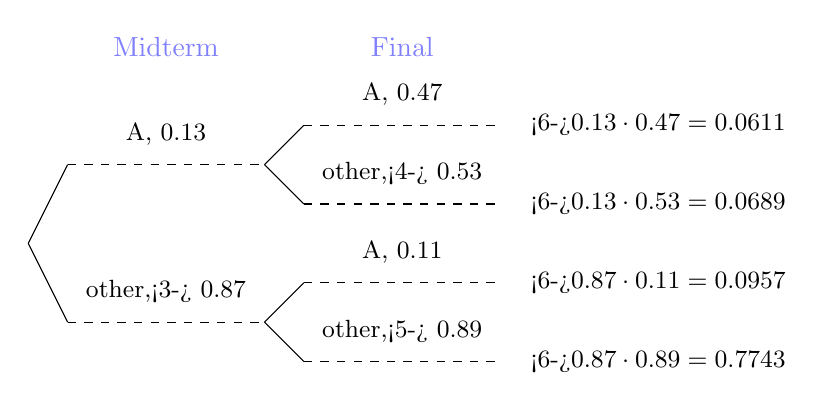
\begin{tikzpicture}
\newcommand{\varA}{\variable{Midterm}}
\newcommand{\varB}{\variable{Final}}
\newcommand{\outAone}{\outcome{A}}
\newcommand{\outAtwo}{\outcome{other}}
\newcommand{\outBone}{\outcome{A}}
\newcommand{\outBtwo}{\outcome{other}}
\newcommand{\outAoneprob}{0.13}
\newcommand{\outAtwoprob}{0.87}
\newcommand{\outAoneBoneprob}{0.47}
\newcommand{\outAoneBtwoprob}{0.53}
\newcommand{\outAtwoBoneprob}{0.11}
\newcommand{\outAtwoBtwoprob}{0.89}

\newcommand{\rowlabel}{2.5}
\newcommand{\rowthreeup}{1.5}
\newcommand{\rowtwoup}{1.0}
\newcommand{\rowoneup}{0.5}
\newcommand{\rowonedown}{-0.5}
\newcommand{\rowtwodown}{-1.0}
\newcommand{\rowthreedown}{-1.5}

\newcommand{\colone}{0.5}
\newcommand{\coltwo}{3}
\newcommand{\colthree}{3.5}
\newcommand{\colfour}{6}
\newcommand{\colfive}{8}

\FPeval\midone{clip((\colone+\coltwo)/2)} % chktex 36
\FPeval\midtwo{clip((\colthree+\colfour)/2)} % chktex 36
\FPeval\ansa{clip(\outAoneprob * \outAoneBoneprob)} 
\FPeval\ansa{round(ansa:4)}
\FPeval\ansb{clip(\outAoneprob * \outAoneBtwoprob)} 
\FPeval\ansb{round(ansb:4)}
\FPeval\ansc{clip(\outAtwoprob * \outAtwoBoneprob)} 
\FPeval\ansc{round(ansc:4)}
\FPeval\ansd{clip(\outAtwoprob * \outAtwoBtwoprob)} 
\FPeval\ansd{round(ansd:4)}

\draw (0,0) -- (\colone, \rowtwoup);
\draw[dashed] (\colone, \rowtwoup) -- (\coltwo, \rowtwoup);
\draw (\coltwo, \rowtwoup) -- (\colthree, \rowthreeup);
\draw[dashed] (\colthree, \rowthreeup) -- (\colfour, \rowthreeup);
\draw (\coltwo, \rowtwoup) -- (\colthree, \rowoneup);
\draw[dashed] (\colthree, \rowoneup) -- (\colfour, \rowoneup);

\draw (0,0) -- (\colone, \rowtwodown);
\draw[dashed] (\colone, \rowtwodown) -- (\coltwo, \rowtwodown);
\draw (\coltwo, \rowtwodown) -- (\colthree, \rowthreedown);
\draw[dashed] (\colthree, \rowthreedown) -- (\colfour, \rowthreedown);
\draw (\coltwo, \rowtwodown) -- (\colthree, \rowonedown);
\draw[dashed] (\colthree, \rowonedown) -- (\colfour, \rowonedown);

\node[label={\small \outAone,~\outAoneprob}] at (\midone,\rowtwoup) {};
\node[label={\small \outAtwo,\blanked<3->{~\outAtwoprob}}] at (\midone,\rowtwodown) {};
\node[label={\small \outBone,~\outAoneBoneprob}] at (\midtwo,\rowthreeup) {};
\node[label={\small \outBtwo,\blanked<4->{~\outAoneBtwoprob}}] at (\midtwo,\rowoneup) {};
\node[label={\small \outBtwo,\blanked<5->{~\outAtwoBtwoprob}}] at (\midtwo,\rowthreedown) {};
\node[label={\small \outBone,~\outAtwoBoneprob}] at (\midtwo,\rowonedown) {};

\node at (\colfive,\rowthreeup) {\small \blanked<6->{$\outAoneprob \cdot \outAoneBoneprob=\ansa$}};
\node at (\colfive,\rowoneup) {\small \blanked<6->{$\outAoneprob \cdot \outAoneBtwoprob=\ansb$}};
\node at (\colfive,\rowonedown) {\small \blanked<6->{$\outAtwoprob \cdot \outAtwoBoneprob=\ansc$}};
\node at (\colfive,\rowthreedown) {\small \blanked<6->{$\outAtwoprob \cdot \outAtwoBtwoprob=\ansd$}};

\node[blue!50] at (\midone, \rowlabel) {\varA};
\node[blue!50] at (\midtwo, \rowlabel) {\varB};
\end{tikzpicture}
}
\end{center}
\onslide<7->
\vspace{-2mm}
\begin{equation*}
\begin{aligned}
\condprob{\text{\small\variable{midterm} is \outcome{A}}}{\text{\small\variable{final} is \outcome{A}}} \onslide<8->
&=\dfrac{\jointprob{\text{\small\variable{midterm} is \outcome{A}}}{and}{{\text{\small\variable{final} is \outcome{A}}}}}{\prob{{\text{\small\variable{final} is \outcome{A}}}}}\\\onslide<9->
&=\dfrac{0.0611}{0.1568} \onslide<10->
= 0.3897 \approx 38.97\%
\end{aligned}
\end{equation*}
\end{example}
\end{frame}

\begin{frame}
\begin{definition}
A \textbf{false negative} is when a test incorrectly gives a negative result.
\end{definition}\pause

\begin{definition}
A \textbf{false positive} is when a test incorrectly gives a positive result.
\end{definition}\pause

\begin{example}
In Canada, about 0.35\% of women over 40 will develop breast cancer in any given year. A common screening test for cancer is the mammogram, but this test is not perfect.\pause

\vspace{2mm}
In about 11\% of patients with breast cancer, the test gives a false negative. That is, the mammogram indicated the woman does not have breast cancer, when she really does have breast cancer.\pause

\vspace{2mm}
In about 7\% of patients that do not have breast cancer, the test gives a true negative. That is, the mammogram indicated the woman does have breast cancer, when she really doesn't have breast cancer.
\end{example}
\end{frame}

\begin{frame}
\begin{example}\label{canadian breast cancer}
\vspace{-2mm}%beamer bug: extra space is added when a label is used, so this is to make this slide and the next look the same
A question doctors and researchers have to answer is: If the mammogram comes back positive, what is the probability that the patient actually has breast cancer?\pause

\vspace{1mm}
We have enough information to build a tree diagram:

\vspace{-2.5mm}
\begin{center}
\scalebox{0.75}{%
\begin{tikzpicture}
\newcommand{\varA}{\variable{Truth}}
\newcommand{\varB}{\variable{Mammogram}}
\newcommand{\outAone}{\outcome{cancer}}
\newcommand{\outAtwo}{\outcome{no cancer}}
\newcommand{\outBone}{\outcome{positive}}
\newcommand{\outBtwo}{\outcome{negative}}
\newcommand{\outAoneprob}{0.0035}
\newcommand{\outAtwoprob}{0.9965}
\newcommand{\outAoneBoneprob}{0.89}
\newcommand{\outAoneBtwoprob}{0.11}
\newcommand{\outAtwoBoneprob}{0.07}
\newcommand{\outAtwoBtwoprob}{0.93}

\newcommand{\rowlabel}{2.5}
\newcommand{\rowthreeup}{1.5}
\newcommand{\rowtwoup}{1.0}
\newcommand{\rowoneup}{0.5}
\newcommand{\rowonedown}{-0.5}
\newcommand{\rowtwodown}{-1.0}
\newcommand{\rowthreedown}{-1.5}

\newcommand{\colone}{0.75}
\newcommand{\coltwo}{3.75}
\newcommand{\colthree}{4.5}
\newcommand{\colfour}{7}
\newcommand{\colfive}{9.5}

\FPeval\midone{clip((\colone+\coltwo)/2)} % chktex 36
\FPeval\midtwo{clip((\colthree+\colfour)/2)} % chktex 36
\FPeval\ansa{clip(\outAoneprob * \outAoneBoneprob)} 
\FPeval\ansa{round(ansa:5)}
\FPeval\ansb{clip(\outAoneprob * \outAoneBtwoprob)} 
\FPeval\ansb{round(ansb:5)}
\FPeval\ansc{clip(\outAtwoprob * \outAtwoBoneprob)} 
\FPeval\ansc{round(ansc:5)}
\FPeval\ansd{clip(\outAtwoprob * \outAtwoBtwoprob)} 
\FPeval\ansd{round(ansd:5)}

\draw (0,0) -- (\colone, \rowtwoup);
\draw[dashed] (\colone, \rowtwoup) -- (\coltwo, \rowtwoup);
\draw (\coltwo, \rowtwoup) -- (\colthree, \rowthreeup);
\draw[dashed] (\colthree, \rowthreeup) -- (\colfour, \rowthreeup);
\draw (\coltwo, \rowtwoup) -- (\colthree, \rowoneup);
\draw[dashed] (\colthree, \rowoneup) -- (\colfour, \rowoneup);

\draw (0,0) -- (\colone, \rowtwodown);
\draw[dashed] (\colone, \rowtwodown) -- (\coltwo, \rowtwodown);
\draw (\coltwo, \rowtwodown) -- (\colthree, \rowthreedown);
\draw[dashed] (\colthree, \rowthreedown) -- (\colfour, \rowthreedown);
\draw (\coltwo, \rowtwodown) -- (\colthree, \rowonedown);
\draw[dashed] (\colthree, \rowonedown) -- (\colfour, \rowonedown);

\node[label={\small \outAone,~\outAoneprob}] at (\midone,\rowtwoup) {};
\node[label={\small \outAtwo,~\outAtwoprob}] at (\midone,\rowtwodown) {};
\node[label={\small {\color<5>{purple!60}{\outBone}},~\outAoneBoneprob}] at (\midtwo,\rowthreeup) {};
\node[label={\small \outBtwo,~\outAoneBtwoprob}] at (\midtwo,\rowoneup) {};
\node[label={\small \outBtwo,~\outAtwoBtwoprob}] at (\midtwo,\rowthreedown) {};
\node[label={\small {\color<5>{orange!75}{\outBone}},~\outAtwoBoneprob}] at (\midtwo,\rowonedown) {};

\node at (\colfive,\rowthreeup) {\small $\outAoneprob \cdot \outAoneBoneprob=\color<5>{purple!60}{\ansa}$};
\node at (\colfive,\rowoneup) {\small $\outAoneprob \cdot \outAoneBtwoprob=\ansb$};
\node at (\colfive,\rowonedown) {\small $\outAtwoprob \cdot \outAtwoBoneprob=\color<5>{orange!75}{\ansc}$};
\node at (\colfive,\rowthreedown) {\small $\outAtwoprob \cdot \outAtwoBtwoprob=\ansd$};

\node[blue!50] at (\midone, \rowlabel) {\varA};
\node[blue!50] at (\midtwo, \rowlabel) {\varB};
\end{tikzpicture}
}
\end{center}\pause
\vspace{-3mm}
So,

\vspace{-6mm}
\begin{equation*}
\begin{aligned}
\condprob{\text{\small has BC}}{\text{\small test positive}}\pause
&= \dfrac{\jointprob{\text{\small has BC}}{and}{\text{\small test positive}}}{\prob{\text{\small test positive}}}\\\pause
&= \dfrac{\color<5>{purple!60}{0.00312}}{\color<5>{purple!60}{0.00312} + \color<5>{orange!75}{0.06976}} \pause= 0.0428 \approx 4.28\%
\end{aligned}
\end{equation*}
\end{example}
\end{frame}

\newcommand{\bayesterm}[2]{\condprob{#1}{#2}\prob{#2}}
\begin{frame}
\begin{note}
There are times where we are given:

\vspace{-4mm}
\begin{equation*}
\condprob{\text{\small statement about \variable{variable 1|}}}{\text{\small statement about \variable{variable 2}}}
\end{equation*}

\vspace{-1mm}
but we would rather know the inverted conditional probability:

\vspace{-4mm}
\begin{equation*}
\condprob{\text{\small statement about \variable{variable 2}}}{\text{\small statement about \variable{variable 1}}}
\end{equation*}
\end{note}\pause

\begin{block}{Bayes' Theorem}
Consider the following conditional probability for \variable{variable 1} and \variable{variable 2}:

\vspace{-4mm}
\begin{equation*}
\condprob{\text{\small outcome $A_1$ of \variable{variable 1}}}{\text{\small outcome $B$ of \variable{variable 2}}}
\end{equation*}

\vspace{-1mm}
Bayes' Theorem states that this conditional probability is the same as:

\vspace{-2mm}
\begin{equation*}
\dfrac{\bayesterm{B}{A_1}}{\bayesterm{B}{A_1}+\bayesterm{B}{A_2}+\cdots+\bayesterm{B}{A_k}}
\end{equation*}
\small
where $A_2$, $A_3$, \ldots, $A_k$ represent all other possible outcomes of \variable{variable 1}.
\end{block}
\end{frame}

\newcommand{\testpositive}{\text{\small test pos}}
\newcommand{\hasBC}{\text{\small has BC}}
\newcommand{\noBC}{\text{\small no BC}}
\begin{frame}
\begin{example}
In Example~\ref{canadian breast cancer}, we computed $\condprob{\text{\small has BC}}{\text{\small test positive}}$ using a tree diagram.\pause

\vspace{2mm}
We could have also used Bayes' Theorem:
\begin{equation*}
\begin{array}{l}
\condprob{\hasBC}{\testpositive}\\
\quad= \dfrac{\bayesterm{\testpositive}{\hasBC}}{\bayesterm{\testpositive}{\hasBC}+\bayesterm{\testpositive}{\noBC}} \\[4mm]\pause
\quad= \dfrac{0.89\cdot 0.0035}{0.89\cdot0.0035 + 0.07\cdot 0.9965} \pause = \dfrac{0.03115}{0.07287} \pause = 0.0428 \approx 4.28\%
\end{array}
\end{equation*}
\end{example}\pause

\begin{note}
This strategy of updating beliefs using Bayes' Theorem is the foundation of an entire branch of statistics called \textbf{Bayesian statistics}.
\end{note}
\end{frame}
\end{document}